%!TEX root = ../main.tex
\section{Các nghiên cứu liên quan}
\begin{frame}{MFEA - giải số lượng tác vụ nhỏ}
    \begin{block}{MFEA}
        \begin{itemize}
            \item \fullcite{gupta2015multifactorial}
            \item \textbf{Vấn đề:} Lai ghép khác tác vụ một cách ngẫu nhiên.
        \end{itemize}
    \end{block}
    \begin{block}{MFEA-II}
        \begin{itemize}
            \item \fullcite{bali2019multifactorial}
            \item \textbf{Ý tưởng:} Giải quyết bài toán con (tối ưu hàm lồi), tối ưu $RMP \in \mathbb{R}^{K \times K}$ sao cho con sinh ra từ quần thể cha mẹ và $RMP$ giống với con được chọn lọc sang thế hệ tiếp theo nhất.
            \item \textbf{Vấn đề:} Thuật toán chạy chậm, khi phải giải quyết $K^2$ bài toán con.
        \end{itemize}
    \end{block}
\end{frame}


\begin{frame}{MFEA - giải số lượng tác vụ lớn}
    \begin{block}{GMFEA}
        \begin{columns}
            \begin{column}{0.64\textwidth}
                \begin{itemize}
                    \item \fullcite{tang2018group}
                    \item Với mỗi tác vụ, chọn một vài cá thể tốt nhất làm đại diện, gộp lại thành một tập dữ liệu
                    \item Dùng thuật toán K-Means, nhóm dữ liệu trên lại.
                    \item Các tác vụ ở cùng một cụm mới được trao đổi thông tin cho nhau.
                    \item \textbf{Vấn đề:} trường hợp quần thể cùng phân phối nhưng cần đi về khác hướng (Hình \ref{fig:related:similar-distribution}).
                \end{itemize}
            \end{column}
            \begin{column}{0.34\textwidth}
                \begin{figure}
                    \centering
                    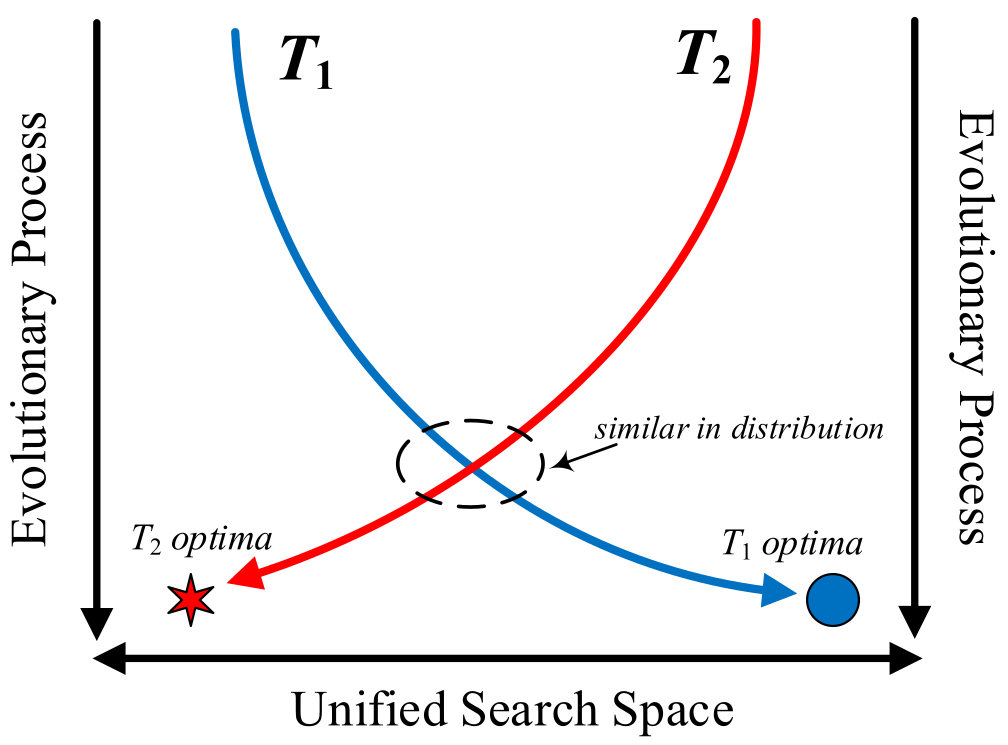
\includegraphics[width=\linewidth]{figure/related/similar_distribution.png}
                    \caption{\fontsize{8pt}{10}\selectfont Hai tác vụ cùng vị trí quần thể, khác vị trí cực trị.}
                    \label{fig:related:similar-distribution}
                \end{figure}
            \end{column}
        \end{columns}
    \end{block}
\end{frame}

\begin{frame}{MFEA - giải số lượng tác vụ lớn}
    \begin{block}{SBSGA}
        \begin{itemize}
            \item \fullcite{liaw2019evolutionary}
            \item Trao đổi thông tin giữa các tác vụ bằng việc tráo cá thể (swap) thay vì lai ghép.
            \item Lưu lại số lần trao đổi thành công $T^{pos}$ (con được chọn lọc vào quần thể mới) và thất bại $T^{neg}$.
            \item Xác suất trao đổi tính bằng công thức: 
                \begin{equation}
                    RMP_{i, j} = \frac{T^{pos}}{T^{pos} + T^{neg}}
                \end{equation}
            \item \textbf{Vấn đề:} Phương pháp ghép cặp tự thiết kế không dựa trên lý thuyết.
        \end{itemize}
    \end{block}
\end{frame}

\begin{frame}{MFEA - giải số lượng tác vụ lớn}
    \begin{block}{MaTGA}
        \begin{itemize}
            \item \fullcite{chen2019adaptive}
            \item Lưu một phần quần thể của từng tác vụ qua nhiều thế hệ.
            \item Tính khoảng cách KL Divergence giữa các tập quần thể đã lưu.
            \item \textbf{Vấn đề:} Có nhiều tham số, thời gian tính toán chậm.
        \end{itemize}
    \end{block}
\end{frame}
